\usetikzlibrary{arrows.meta,calc}
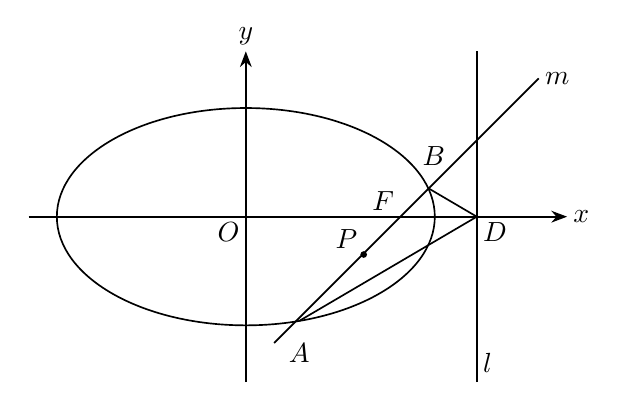
\begin{tikzpicture}[x=1.2cm,y=1.2cm,line width=.6pt,>=Stealth,font=\normalsize]
\coordinate (O) at (0.00000000,0.00000000);
\coordinate (F) at (1.63630682,0.00000000);
\coordinate (A) at (0.56533538,-1.10310058);
\coordinate (B) at (1.92970841,0.30220364);
\coordinate (P) at (1.24752189,-0.40044847);
\coordinate (D) at (2.44452933,0.00000000);
\coordinate (M1) at (0.30000000,-1.33630682);
\coordinate (M2) at (3.10000000,1.46369318);
\coordinate (Lbot) at (2.44452933,-1.75000000);
\coordinate (Ltop) at (2.44452933,1.75000000);
\coordinate (Xleft) at (-2.30000000,0.00000000);
\coordinate (Xright) at (3.40000000,0.00000000);
\coordinate (Ybot) at (0.00000000,-1.75000000);
\coordinate (Ytop) at (0.00000000,1.75000000);
\draw[->] (Xleft)--(Xright);
\draw[->] (Ybot)--(Ytop);
\draw (O) ellipse [x radius=2.00000000,y radius=1.15000000];
\draw (M1)--(M2);
\draw (A)--(D)--(B);
\draw (Lbot)--(Ltop);
\fill (P) circle (1.2pt);
\node[below left,inner sep=0pt,xshift=-2pt,yshift=-2pt] at (O) {$O$};
\node[above left,inner sep=0pt,xshift=-2pt,yshift=2pt] at (F) {$F$};
\node[below,inner sep=0pt,yshift=-8pt] at (A) {$A$};
\node[above,inner sep=0pt,xshift=2pt,yshift=8pt] at (B) {$B$};
\node[above left,inner sep=0pt,xshift=-2pt,yshift=2pt] at (P) {$P$};
\node[below right,inner sep=0pt,xshift=2pt,yshift=-2pt] at (D) {$D$};
\node[right,inner sep=0pt,xshift=2pt] at (M2) {$m$};
\node[right,inner sep=0pt,xshift=2pt] at (2.44452933,-1.55) {$l$};
\node[right,inner sep=0pt,xshift=2pt] at (Xright) {$x$};
\node[above,inner sep=0pt,yshift=2pt] at (Ytop) {$y$};
\end{tikzpicture}
